\documentclass[11pt]{article}
\usepackage{arxiv}

\title{CACTUS: Combinatorial Action Masking for Tool-Augmented Sequential Reasoning}

\author{
  Pranith \\
  IIT Bombay \\
  \texttt{pranith@minds.iitb.ac.in} \\
}

\begin{document}
\maketitle

\begin{abstract}
Large Language Models (LLMs) can invoke external tools, but selecting the exact subset of tools a multi-hop query requires remains difficult: zero-shot prompting reliably over-predicts, appending plausible-but-unnecessary tools that accumulate downstream errors. We introduce CACTUS, which formulates tool selection as a sequential Markov Decision Process and solves it with Proximal Policy Optimization under strict autoregressive action masking. The mask removes each selected tool from the action space, which makes repeated selections impossible by construction and bounds every trajectory to at most $|\mathcal{A}|$ steps. On a 15-tool benchmark derived from MetaTool, CACTUS attains a sequence exact-match rate of $0.573 \pm 0.067$ across five training seeds, against $0.255$ for zero-shot LLaMA-3.1-8B-Instruct and $0.137$ for a validation-calibrated dense-retrieval baseline --- a paired improvement over the LLM of $+0.318$ (95\% CI $[0.184, 0.451]$, Wilcoxon $p = 7.0\times10^{-5}$). Notably, the picture differs by metric: on token-level F1, CACTUS ($0.806 \pm 0.031$) is only marginally ahead of the 8B LLM ($0.744$, $p = 0.059$, not significant), because an over-predicting model still earns substantial partial credit. Our results indicate that the benefit of RL-driven action masking lies specifically in emitting exactly the right tool set, not in broad token-level accuracy, and that a policy with roughly four orders of magnitude fewer parameters suffices to obtain it.
\end{abstract}

\section{Introduction}
The integration of external tools has transformed Large Language Models (LLMs) from passive text generators into active agents \cite{mialon2023augmented, karpas2022mrkl}. By interfacing with search engines, calculators, and proprietary databases, tool-augmented LLMs address multi-hop tasks that exceed their parametric memory \cite{schick2023toolformer}. As the vocabulary of available tools grows, however, routing a query to the correct subset of tools becomes progressively harder \cite{qin2023toolllm}.

The difficulty is combinatorial. A query requiring several distinct operations forces the agent to search a space of size $\mathcal{O}(\binom{N}{K})$ to identify the exact subset needed. Two paradigms dominate. Dense retrieval treats selection as semantic matching, scoring each tool independently against the query; this discards the sequential dependencies between tools and, lacking any notion of sufficiency, provides no principled stopping rule. Zero-shot LLM planning \cite{yao2022react} instead generates tool names directly, but degrades in a specific and measurable way: it \emph{over-predicts}. In our evaluation, LLaMA-3.1-8B-Instruct \cite{dubey2024llama3} emits a superset of the required tools on the majority of queries, which preserves recall while depressing precision and, critically, rarely produces the exact set an execution pipeline needs.

\begin{figure}[t]
\centering
\begin{tikzpicture}[node distance=2.5cm, auto, thick]
\tikzstyle{block} = [rectangle, draw, fill=blue!10, text width=6em, text centered, rounded corners, minimum height=3em]
\tikzstyle{rlblock} = [rectangle, draw, fill=green!10, text width=6em, text centered, rounded corners, minimum height=3em]
\tikzstyle{maskblock} = [rectangle, draw, fill=red!10, text width=6em, text centered, rounded corners, minimum height=3em]
\tikzstyle{line} = [draw, -latex']

\node [block] (query) {User Query $q$};
\node [block, right of=query, node distance=3.5cm] (encoder) {Embedding $E(q)$};
\node [rlblock, right of=encoder, node distance=3.5cm] (ppo) {PPO Policy $\pi_\theta(a_t | s_t)$};
\node [maskblock, below of=ppo, node distance=2cm] (mask) {Action Mask $\mathbf{m}_t$};
\node [block, right of=ppo, node distance=3.5cm] (env) {Tool Env (Execute $a_t$)};

\path [line] (query) -- (encoder);
\path [line] (encoder) -- (ppo);
\path [line] (ppo) -- (env);
\path [line] (env.south) |- node[near start, right] {Update History $\mathbf{h}_{t+1}$} (mask.east);
\path [line] (mask) -- node[left] {Prune Space} (ppo);
\end{tikzpicture}
\caption{CACTUS selects tools one at a time under a mask that deletes every previously chosen tool from the action space. Because the mask strictly shrinks the legal action set at each step, repeated selections are impossible by construction and every trajectory terminates within $|\mathcal{A}|$ steps --- the agent must either choose a new tool or stop. Empirically this yields exact tool sets on $57.3\%$ of held-out queries versus $25.5\%$ for zero-shot LLaMA-3.1-8B-Instruct.}
\label{fig:architecture}
\end{figure}

We formalize combinatorial tool selection as a sequential Markov Decision Process (MDP) and train a policy to navigate it with Reinforcement Learning. \textbf{CACTUS} (\textbf{C}ombinatorial \textbf{A}ction Masking for \textbf{C}omplex \textbf{T}ool \textbf{U}tilization \textbf{S}equences), illustrated in Figure~\ref{fig:architecture}, couples Proximal Policy Optimization (PPO) \cite{schulman2017ppo} with strict autoregressive action masking. The mask is enforced inside the policy's action distribution, not merely encouraged by a reward penalty: already-selected tools receive exactly zero probability mass, so redundant selections cannot occur and trajectory length is bounded a priori.

Our contributions are:
\begin{itemize}
    \item We formalize complex tool selection as a sequential MDP whose state is the query embedding paired with a binary selection history, and show that enforcing an autoregressive mask over this history bounds trajectory length to $T \le |\mathcal{A}|$ by construction.
    \item We implement CACTUS with masked PPO and evaluate it under a protocol designed to be falsifiable: five independent training seeds, a deterministic single pass over every held-out example, and baselines given stopping rules calibrated on validation data.
    \item We show the gain is metric-specific. CACTUS more than doubles exact-match success over a zero-shot 8B LLM ($0.573 \pm 0.067$ vs.\ $0.255$; $p = 7.0\times10^{-5}$) while its F1 advantage over the same model is not statistically significant ($p = 0.059$) --- evidence that masking buys set-level exactness rather than general accuracy.
\end{itemize}

\section{Related Work}
\textbf{Tool-Augmented Large Language Models.} Frameworks such as Toolformer \cite{schick2023toolformer}, HuggingGPT \cite{shen2023hugginggpt}, and Gorilla \cite{patil2023gorilla} show that language models can be fine-tuned or prompted to emit API calls, while ReAct \cite{yao2022react} interleaves chain-of-thought planning with tool execution. These approaches rely on few-shot prompting or supervised fine-tuning, and because they generate tool names as free text they have no structural mechanism preventing a tool from being emitted twice or a plan from running long. As tool vocabularies grow, zero-shot planners increasingly over-predict \cite{qin2023toolllm}. Our contribution is orthogonal to the choice of backbone: we change the \emph{decision procedure}, replacing free-form generation with a constrained sequential policy.

\textbf{Retrieval-Augmented Tool Selection.} To handle large tool vocabularies, prior work retrieves candidate tools by embedding similarity. Retrieval is efficient but treats tools as independent documents, capturing neither conditional dependencies nor a criterion for when enough tools have been gathered. We make this concrete: our dense-retrieval baseline is only competitive once we equip it with an explicit similarity-threshold stopping rule tuned on validation data (Section~\ref{sec:protocol}), and even then it trails a learned policy substantially.

\textbf{Reinforcement Learning for Autonomous Agents.} RL applied to LLMs has largely targeted alignment (RLHF) or web-navigation tasks. CACTUS instead applies RL to the combinatorial structure of multi-tool selection, using action masking --- standard in board-game and combinatorial-optimization agents --- to encode the constraint that a tool is selected at most once.

\section{CACTUS: Methodology}
We formalize LLM-guided sequential tool selection as a discrete-time Markov Decision Process (MDP).

\subsection{MDP Formulation}
The environment is the tuple $\mathcal{M} = \langle \mathcal{S}, \mathcal{A}, \mathcal{P}, \mathcal{R}, \rho_0, \gamma \rangle$.

\textbf{State Space ($\mathcal{S}$).}
A state $s_t = (E(q), \mathbf{h}_t)$, where $E(q) \in \mathbb{R}^{384}$ is a dense embedding of the query $q$ from a frozen \textit{all-MiniLM-L6-v2} encoder, and $\mathbf{h}_t \in \{0,1\}^{|\mathcal{A}|}$ is a binary vector recording which tools have been selected so far.

\textbf{Action Space ($\mathcal{A}$).}
$\mathcal{A} = \{a^{(1)}, \dots, a^{(N)}\} \cup \{a_{\text{TERM}}\}$, where $N$ is the tool-vocabulary size and $a_{\text{TERM}}$ (``DONE'') ends the episode. In our benchmark $N = 15$, so $|\mathcal{A}| = 16$.

\textbf{Transition Dynamics ($\mathcal{P}$).}
Transitions are deterministic. For any $a_t \neq a_{\text{TERM}}$ the history updates as $\mathbf{h}_{t+1} = \mathbf{h}_t \vee \mathbf{e}_{a_t}$, where $\mathbf{e}_{a_t}$ is the standard basis vector for the chosen tool. We emphasize that this update applies whether or not the selected tool was correct: an incorrect choice still consumes that action, which is what makes the length bound in Section~\ref{sec:masking} hold unconditionally.

\textbf{Reward Function ($\mathcal{R}$).}
Let $\mathcal{T}^*(q)$ be the ground-truth tool set and $\mathcal{T}_t(q)$ the set selected up to time $t$. With step penalty $\eta = 0.05$:
\begin{equation}
\mathcal{R}(s_t, a_t) =
\begin{cases}
r_{\text{correct}} - \eta, & a_t \in \mathcal{T}^*(q) \setminus \mathcal{T}_t(q) \\
r_{\text{incorrect}} - \eta, & a_t \notin \mathcal{T}^*(q) \\
\beta, & a_t = a_{\text{TERM}},\ \mathcal{T}_t(q) = \mathcal{T}^*(q) \\
\text{F1}(\mathcal{T}_t(q), \mathcal{T}^*(q)), & a_t = a_{\text{TERM}},\ \text{otherwise}
\end{cases}
\end{equation}
with $r_{\text{correct}} = 1.0$, $r_{\text{incorrect}} = -0.5$, and an exact-match terminal bonus $\beta = 2.0$. The bonus is strictly larger than the best achievable partial-credit terminal reward ($\text{F1} < 1$ whenever $\mathcal{T}_t \neq \mathcal{T}^*$), so the optimal policy prefers stopping on the exact set over accumulating partial credit. There is no redundant-selection case: masking makes it unreachable.

\subsection{Policy Optimization and Action Masking}
\label{sec:masking}
Let $\pi_\theta(a_t | s_t)$ be a stochastic policy optimized with PPO \cite{schulman2017ppo}. Define the mask $\mathbf{m}_t \in \{0,1\}^{|\mathcal{A}|}$ by $m_{t,i} = 1 - h_{t,i}$ for tool actions, with $m_{t,\text{TERM}} = 1$ always. The policy acts under the renormalized distribution
\begin{equation}
\tilde{\pi}_\theta(a_i | s_t) = \frac{\pi_\theta(a_i | s_t) \cdot m_{t, i}}{\sum_{j=1}^{|\mathcal{A}|} \pi_\theta(a_j | s_t) \cdot m_{t, j}}.
\end{equation}
The mask is applied to the logits before sampling, both during rollouts and at evaluation time, so masked actions receive exactly zero probability rather than a learned penalty.

\textbf{Trajectory bound.} Since $\mathbf{h}_t$ gains a set bit on every non-terminating step and no bit is ever cleared, at most $N$ such steps can occur; after that $a_{\text{TERM}}$ is the only unmasked action. Hence every trajectory satisfies $T \le N + 1 = |\mathcal{A}|$, independent of the policy parameters and without relying on a step limit. Cyclic behaviour --- an agent oscillating between tools until truncation, the dominant failure mode of unconstrained sequential agents --- cannot occur.

\section{Experiments}

\subsection{Benchmark}
We evaluate on a multi-tool query benchmark derived from MetaTool \cite{huang2024metatool}, comprising 497 natural-language queries annotated with the exact set of tools required, over a vocabulary of 15 tools. We split 397/49/51 into train/validation/test. The validation split is used exclusively for baseline calibration and the test split exclusively for the reported numbers.

We note one property of this benchmark explicitly, because it bounds how far our conclusions generalize: \emph{every} query in it requires exactly two tools, so $|\mathcal{T}^*(q)| = 2$ throughout and the target space is the $\binom{15}{2} = 105$ two-element subsets. The cardinality is therefore constant and, in principle, learnable --- a point we return to in Limitations.

\subsection{Evaluation Protocol}
\label{sec:protocol}
Three design choices make the comparison falsifiable:

\textbf{Multiple seeds.} CACTUS is trained five times with independent seeds ($42$--$46$); we report mean $\pm$ standard deviation across seeds. The stochastic Random baseline is likewise repeated five times.

\textbf{Deterministic, matched evaluation.} Every agent is evaluated with a single ordered pass over all 51 test queries, visiting each exactly once. All agents therefore see identical episodes, which makes per-example comparisons paired.

\textbf{Baselines with stopping rules.} An agent that cannot stop is not a fair comparison for one that can, since it is forced to keep adding tools past the correct set and forfeit precision. We therefore give Dense Retrieval an explicit stopping rule: it selects the highest-similarity unselected tool until the best remaining cosine similarity falls below a threshold. That threshold is swept on the \emph{validation} split (selected value $0.175$, validation F1 $0.665$) and then frozen. The heuristic baseline stops when no unmatched tool name appears in the query.

\subsection{Metrics}
\textbf{Sequence Exact Match (SEM):} $\mathbb{I}[\mathcal{T}_{T}(q) = \mathcal{T}^*(q)]$, the fraction of queries where the emitted set is exactly right.
\textbf{F1:} harmonic mean of precision and recall over selected tools, awarding partial credit.
\textbf{Trajectory Length (TL):} steps taken before $a_{\text{TERM}}$.

\subsection{Implementation and Compute}
CACTUS uses MaskablePPO (\textit{sb3-contrib}) with a \texttt{MultiInputPolicy} over the (embedding, history) observation: learning rate $3\times10^{-4}$, $\gamma = 0.99$, batch size $64$, $10^5$ timesteps per seed. The sentence encoder is frozen; only the policy and value heads are trained. Each seed trains in roughly $101$ seconds on a single NVIDIA RTX PRO 6000 Blackwell Max-Q, for a total experimental cost of under $10$ GPU-minutes for all five seeds. The LLaMA-3.1-8B-Instruct baseline is evaluated zero-shot with greedy decoding.

\subsection{Results}

\begin{table}[h]
\centering
\caption{Results on the held-out test split (51 queries). CACTUS and Random report mean $\pm$ std over five seeds; deterministic methods report a single pass. CACTUS attains the highest exact-match rate by a wide margin, while LLaMA-3.1-8B remains competitive on partial-credit F1.}
\label{tab:main_results}
\begin{tabular}{lccc}
\toprule
\textbf{Agent} & \textbf{SEM ($\uparrow$)} & \textbf{F1 ($\uparrow$)} & \textbf{TL ($\downarrow$)} \\
\midrule
\textit{Non-Learning Baselines} \\
Uniform Random & $0.000 \pm 0.000$ & $0.183 \pm 0.021$ & $8.25 \pm 0.64$ \\
Heuristic Rules & $0.000$ & $0.105$ & $1.16$ \\
Dense Retrieval (\textit{all-MiniLM}, calibrated) & $0.137$ & $0.565$ & $2.80$ \\
\midrule
\textit{LLM Baseline (Zero-Shot)} \\
LLaMA-3.1-8B-Instruct \cite{dubey2024llama3} & $0.255$ & $0.744$ & --- \\
\midrule
\textit{RL Agent} \\
CACTUS (ours) & $\mathbf{0.573 \pm 0.067}$ & $\mathbf{0.806 \pm 0.031}$ & $2.79 \pm 0.08$ \\
\bottomrule
\end{tabular}
\end{table}

Table~\ref{tab:main_results} reports the main comparison, and Figure~\ref{fig:main_results} shows it visually. TL is undefined for the LLM baseline, which emits a set in a single generation rather than stepping through an environment.

\begin{figure}[h]
\centering
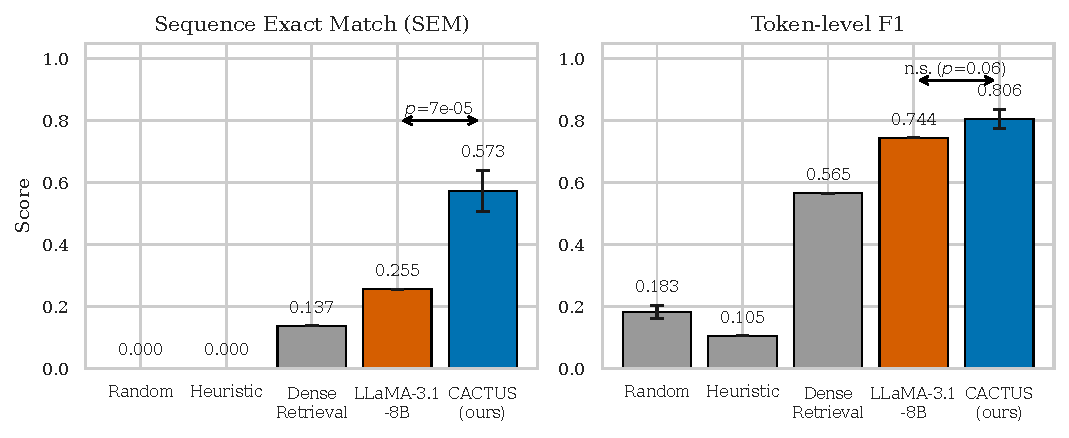
\includegraphics[width=\linewidth]{figures/main_results.pdf}
\caption{The two metrics tell different stories. On exact match (left) CACTUS more than doubles the zero-shot 8B LLM; on token-level F1 (right) the same two systems are statistically indistinguishable. Error bars are one standard deviation across five training seeds (Random: five repeats); deterministic methods have none. This gap between panels, not the absolute height of any bar, is the paper's central result.}
\label{fig:main_results}
\end{figure}

\textbf{Significance.} Table~\ref{tab:significance} reports paired tests over the 51 matched test queries, using CACTUS scores averaged across seeds per example. The exact-match advantage is large and highly significant against every baseline. The F1 advantage over LLaMA-3.1-8B, however, is small and does not reach significance at the $0.05$ level.

\begin{table}[h]
\centering
\caption{Paired comparisons on matched test queries (bootstrap 95\% CI over examples; Wilcoxon signed-rank). The contrast in the final two rows is the paper's central empirical finding: CACTUS's advantage over a zero-shot 8B LLM is decisive on exact match and inconclusive on F1.}
\label{tab:significance}
\begin{tabular}{llcc}
\toprule
\textbf{Comparison} & \textbf{Metric} & \textbf{Diff (95\% CI)} & \textbf{$p$} \\
\midrule
CACTUS vs.\ Random & SEM & $+0.573\ [0.463, 0.686]$ & $2.1\times10^{-8}$ \\
CACTUS vs.\ Random & F1 & $+0.624\ [0.562, 0.683]$ & $5.2\times10^{-10}$ \\
CACTUS vs.\ Dense Retrieval & SEM & $+0.435\ [0.322, 0.553]$ & $3.1\times10^{-7}$ \\
CACTUS vs.\ Dense Retrieval & F1 & $+0.241\ [0.167, 0.317]$ & $8.6\times10^{-7}$ \\
\midrule
CACTUS vs.\ LLaMA-3.1-8B & SEM & $+0.318\ [0.184, 0.451]$ & $7.0\times10^{-5}$ \\
CACTUS vs.\ LLaMA-3.1-8B & F1 & $+0.062\ [0.006, 0.118]$ & $0.059$ (n.s.) \\
\bottomrule
\end{tabular}
\end{table}

\textbf{Interpreting the metric split.} These two results are consistent with a single mechanism, and the per-query predictions confirm it directly. On $33$ of $51$ test queries ($64.7\%$) LLaMA-3.1-8B emits a strict \emph{superset} of the required tools; it emits a strict subset on none. Its predicted sets average $3.27$ tools against a ground truth of $2.00$. Recall is thus nearly saturated --- which is what sustains F1 at $0.74$ --- while the emitted set is rarely exactly right.

CACTUS errs in the opposite direction but less severely, selecting $1.79$ tools on average (trajectories average $2.79$ steps, of which one is the terminating action). Being penalized per step and rewarded for stopping on the exact set, it under-predicts mildly rather than over-predicting heavily, and converts comparable token-level accuracy into far more exactly-correct sets. For a pipeline that executes every predicted tool, this is the distinction that matters: a superset triggers unnecessary calls, latency, and potential side effects, even though F1 scores it favourably. Figure~\ref{fig:mechanism}(a) shows the two distributions directly.

\begin{figure}[h]
\centering
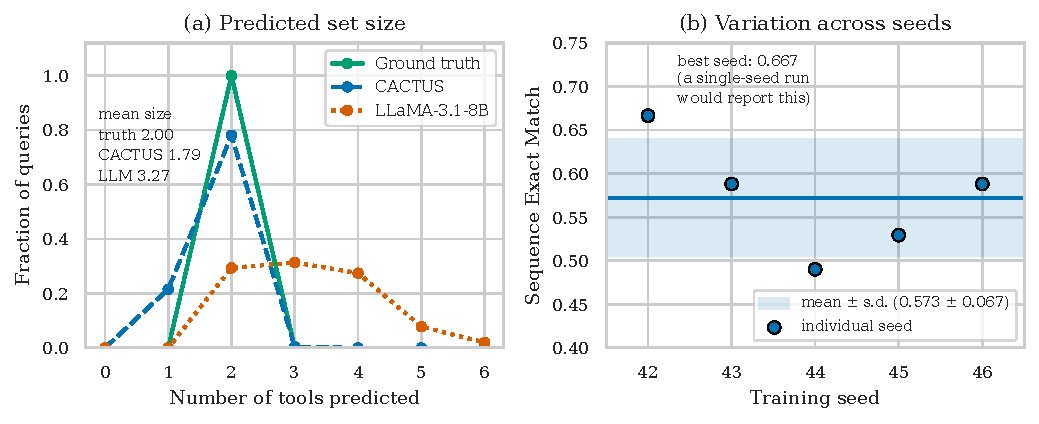
\includegraphics[width=\linewidth]{figures/mechanism.pdf}
\caption{(a) The LLM's predicted-set-size distribution sits to the right of the ground truth (mean $3.27$ vs $2.00$), confirming over-prediction as the failure mode; CACTUS tracks the target distribution closely, erring slightly small. (b) Exact-match varies from $0.490$ to $0.667$ across training seeds, a spread of nearly three standard deviations --- reporting any single run would misstate the method by up to $\pm 0.09$.}
\label{fig:mechanism}
\end{figure}

\textbf{Seed variance.} Per-seed SEM values are $0.667$, $0.588$, $0.490$, $0.529$, and $0.588$. The spread is substantial relative to the effect: the best seed exceeds the worst by $0.177$, nearly three standard deviations. Any single-seed number drawn from this distribution would misrepresent the method by up to $\pm 0.09$, which is why we report the five-seed mean rather than a best run.

\section{Limitations}
\textbf{Scale, and a weaker combinatorial setting than the motivation implies.} Our benchmark has 15 tools, and every query requires exactly two of them, so the effective target space is $\binom{15}{2} = 105$ subsets with known, constant cardinality. This is far milder than the regime that motivates the approach, and it means part of what a policy can learn here is simply ``stop after two tools'' --- a shortcut unavailable when $|\mathcal{T}^*|$ varies. The masking argument (no repeats, bounded trajectories) does not depend on constant cardinality, but our empirical support for it is drawn entirely from a setting where cardinality is fixed. Demonstrating the approach at the scale of ToolBench or ToolLLM's 16{,}000+ APIs \cite{qin2023toolllm}, with variable-size targets, remains open; there a flat masked softmax over actions and a 384-dimensional query embedding are both likely to be inadequate.

\textbf{Test-set size.} With 51 test queries, one additional correct query shifts SEM by $0.02$. Our confidence intervals account for this, but they are wide, and the non-significant F1 comparison against LLaMA would benefit most from a larger evaluation set --- it is plausible that a modest real effect exists there and we are underpowered to detect it.

\textbf{Single dataset and single LLM baseline.} All results come from one MetaTool-derived benchmark and one open-weight model at one size. We have not tested transfer to unseen tool vocabularies, nor compared against larger or tool-specialized LLMs, which may close the exact-match gap.

\textbf{Supervision assumptions.} The reward function requires a ground-truth tool set per query, so CACTUS as presented requires labelled data and does not directly apply to settings where tool utility must be inferred from downstream task success. The frozen encoder also means the policy cannot adapt its query representation.

\textbf{Ordering.} Although CACTUS produces tools sequentially, our metrics evaluate the resulting \emph{set}. We therefore do not claim the learned ordering is itself meaningful.

\section{Conclusion}
We presented CACTUS, which casts combinatorial tool selection as an MDP and solves it with PPO under strict autoregressive action masking. The mask makes redundant selection structurally impossible and bounds trajectory length by construction. Across five seeds, CACTUS emits the exactly-correct tool set on $57.3\%$ of held-out queries, more than double the $25.5\%$ of zero-shot LLaMA-3.1-8B-Instruct, at a training cost under ten GPU-minutes. The advantage is specific rather than general: on partial-credit F1 the two are statistically indistinguishable, and it is set-level exactness --- the property an execution pipeline actually depends on --- where the constrained policy wins. Extending this to large tool vocabularies, where a flat masked action space will not suffice, is the natural next step.

\bibliographystyle{plainnat}
\bibliography{references}

\end{document}
